\documentclass{standalone}


\usepackage{tikz}
\usepackage{pgfplots}
\pgfplotsset{compat=1.15}
\usetikzlibrary{shapes,arrows}
\begin{document}


% The block diagram code is probably more verbose than necessary
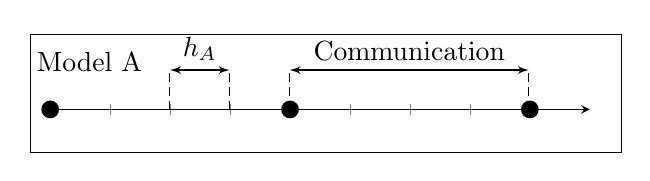
\begin{tikzpicture}[auto, node distance=3cm,>=latex']


\begin{axis}[
    xmin=0, xmax=9,
    axis x line=bottom,% only show the bottom x axis
    hide y axis,    
    ymin=0,ymax=2,
    scatter/classes={%
        a={mark=o,draw=black}},
				xticklabels={,,},
				xtick={1,2,3,5,6,7}
    ]

\addplot[scatter,only marks,
    mark size = 3pt,
    fill = black,
    scatter src=explicit symbolic]
table {
0 0 
4 0 
8 0 
 
    };
\end{axis}
\node at (3.5,0.2) [rectangle,draw,minimum width=7.5cm, minimum height = 1.5cm] (modela) {};
\node at (0.5,0.6) {Model A};
\draw [densely dashed] (1.52,0) -- (1.52,0.5);
\draw [densely dashed] (2.28,0) -- (2.28,0.5);
\draw [densely dashed] (3.04,0) -- (3.04,0.5);
\draw [densely dashed] (6.08,0) -- (6.08,0.5);
\draw[<->] (1.52,0.5) -- node {$h_A$} (2.28,0.5);
\draw[<->] (3.04,0.5) -- node {Communication} (6.08,0.5);




%\begin{axis}[
    %xmin=0, xmax=9,
    %axis x line=bottom,% only show the bottom x axis
    %hide y axis,    
    %ymin=0,ymax=2,
    %scatter/classes={%
        %a={mark=o,draw=black}},
				%xticklabels={,,},
				%xtick={0.5,1,1.5,2,2.5,3,3.5,4.5,5,5.5,6,6.5,7}
    %]
%
%\addplot[scatter,only marks,
    %mark size = 3pt,
    %fill = black,
    %scatter src=explicit symbolic]
%table {
%0 0 
%4 0 
%8 0 
 %
    %};
%\end{axis}

   
\end{tikzpicture}

\end{document}